\documentclass[10pt, a4paper]{article}

% On écrit en français
\usepackage[utf8]{inputenc}
\usepackage[frenchb]{babel}
\usepackage[T1]{fontenc}

% Packages nécessaires
\usepackage{graphicx}
\usepackage{hyperref}

% Numérotation de page custom
\usepackage{fancyhdr}
\usepackage{lastpage}
\pagestyle{fancy}
\fancyhf{}
\rfoot{Page \thepage \hspace{1pt} sur \pageref{LastPage}}

% Police Helvetica <3
\usepackage{helvet}
\renewcommand*{\familydefault}{\sfdefault}

% Enlever les alinéas
\setlength{\parindent}{0pt}

% Marges plus larges pour faire moins LaTeX
\usepackage[left=3cm, right=3cm]{geometry}

% Sous titre de document
\usepackage{titling}
\newcommand{\subtitle}[1]{%
  \posttitle{%
    \par\end{center}
    \begin{center}\large#1\end{center}
    \vskip0.5em}%
}

% En tête complet de document
\newcommand{\Document}[1]{%
    \title{#1}
    \subtitle{Dématérialisation d'un processus de paiement}
    \author{
        COMETS Jean-Marie \\
        DELMARRE Adrian \\
        REYNOLDS Nicolas \\
        TURPIN Pierre
    }
    \date{\today}

    \maketitle \newpage

    \tableofcontents \newpage
}


\begin{document}

\Document{Business plan}

\section{Executive Summary}
Le \textbf{marché du titre de restauration} connaît depuis deux ans une
\textbf{transformation radicale}, avec l’arrivée des titres dématérialisés. La
configuration du marché entraîne une domination solide d’un petit nombre
d’A-Players. Cette transformation est la \textbf{dernière occasion de la
décennie} de se tailler une part dans ce marché de 5.7 milliards d’euros. \\

La France est en retard dans cette transformation, qui est terminée dans
plusieurs pays. Nous avons donc une \textbf{vision très précise} des phases qui
sont à venir, avec notamment le constat suivant : \textbf{des acteurs arrivant
sur le marché ont réussi à se tailler une part}, malgré les réponses des
A-Players, et ce a plusieurs reprises. Il y a donc \textbf{une faille} dans
leurs barrières à l’entrée. En France, d’après les évolutions des marchés
étrangers, il reste 1 ou 2 places à prendre, et 2 ans avant que le marché soit
bloqué. \\

La faille est la suivante : malgré leur énorme puissance financière et la
protection que leur offre leur réseau, les A-Players doivent gérer leur lourde
structure titres-papier, la transition prenant 5 à 7 ans. Ils ne peuvent donc
pas s’aligner sur une \textbf{politique agressive de conquête de marché} qui
joue à la fois sur les \textbf{coûts et sur la rapidité}. \\

Nous proposons de reprendre les éléments qui ont fait le succès des nouveaux
arrivants : \\
\begin{enumerate}
  \item \textbf{Différenciation radicale par les coûts} (0 commission), soutenu par la
    réduction des coûts entraînée par le 100\% dématérialisé.
  \item \textbf{Investir activement nos partenaires clés} dans la conquête de marché :
    prendre le monopole chez nos partenaires grande distribution, s’appuyer sur
    la portée et la puissance financière de la banque.
  \item Se lancer dans une \textbf{conquête rapide et globale} du marché. 
\end{enumerate}
~\\

Une fois placés sur le marché, se diriger vers des \textbf{espaces stratégiques
à plus forte valeur ajoutée} : la vente de produits annexes, marché à la
croissance annuelle de 4\%.  \\

\section{Problème / Opportunité}

Le \textbf{marché du titre de restauration} connaît depuis deux ans une
\textbf{transformation radicale}, avec l’arrivée des titres dématérialisés.
D’autres pays ont entamé avec succès cette transition avant nous, ce qui a
résulté en l’\textbf{arrivée percutante de nouveaux acteurs} sur le marché. Des
places similaires sont donc à prendre en France. Dans cette partie, nous allons
faire un \textbf{état des lieux de la configuration et de l’évolution des
marchés}. \\

\subsection{L’étranger : des transformations terminées}

\subsubsection{Brésil}

Le Brésil est le cas de référence d’un marché qui a \textbf{terminé sa
transition} a des formats dématérialisés. \\

Son étude permet de dégager des effets importants sur le marché : \\
\begin{itemize}
  \item \textbf{Une augmentation du volume total} des transactions
  \item Une compétitivité accrue des acteurs dématérialisés grâce à des
    \textbf{économies d’échelle}
  \item \textbf{Nouvelles sources de revenus} uniques au modèle de la
    carte-restaurant (produits annexes)
  \item Durée totale de la transition d’un pays : \textbf{5 à 7 ans}, avec un
    pic d’adoption en 3 ou 4 ème année
\end{itemize}

\subsubsection{Inde}

L’Inde est un exemple d’implantation réussie de nouveaux acteurs. \\

Le groupe \textbf{Sodexo}, historiquement majoritaire sur le marché, n’a pas pu
contenir l’arrivée de GoBindas, acteur national de taille moyenne. \\

\textbf{GoBindas} est spécialisé dans l’ajout de services pour les opérateurs
télecoms. Il a effectué avec succès une entrée dans le marché du titre de
restauration dématérialisé en 2011, avec solution sur téléphone. \\

Notre analyse des facteurs clés qui ont fait son succès : \\
\begin{description}
  \item[Différenciation par les coûts :] le 100\% dématérialisé lui a permis de
    réduire drastiquement ses coûts de fonctionnement, en opposition à Sodexo. La
    solution par téléphone (SMS notamment), cohérente avec le marché Indien, lui
    a permis une adoption sans friction par les entreprises et les commerces.
  \item[Des partenaires clé puissants :] l’entreprise a noué des partenariats
    avec 500 marques clés (détenues par une poignée de groupes), de manière à lui
    donner une forte visibilité pour s’ancrer dans le marche. Sa proximité avec
    les \textit{acteurs de la télécommunication} lui a permis de mettre en place
    une infrastructure adaptée, ainsi qu’une couverture forte lors de la phase de
    déploiement (groupe TIAXA). 
  \item[Une conquête rapide et globale du marché :] le timing du lancement de ses
    produits a été décisif : Le 1er Janvier, plusieurs acteurs majeurs de la
    grande distribution du pays (Food Bazarn, Spencer's Foodworld etc.) se sont
    mis simultanément à \textit{ne plus accepter les tickets Sodexo}, ce qui lui
    a permis de récupérer une part de marché estimée à 30\% en moins de 6 mois.
\end{description}
~\\

Nous reprendrons ces facteurs de succès pour notre stratégie (cf. Ventes \&
Marketing). \\

\subsection{La France : une transition en démarrage}

% \begin{landscape}
  \begin{figure}[htpb]
      \centering
      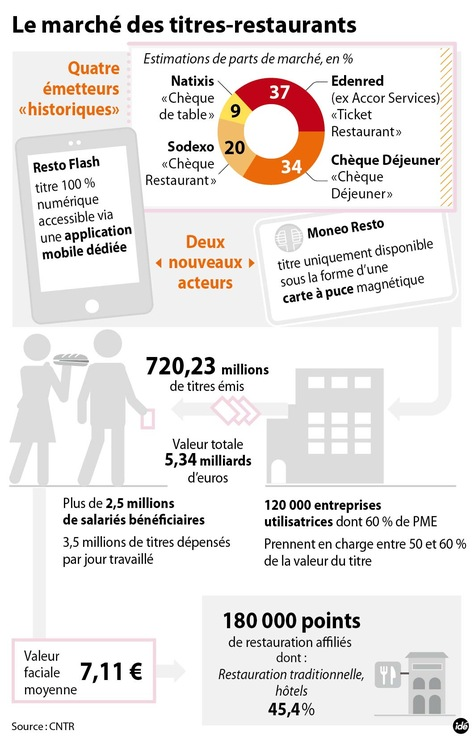
\includegraphics[width=0.8\textwidth]{image06}
      \caption{Vue d’ensemble du marché Français des titres restaurants, réalisée par le CNTR}
      \label{fig:image06}
  \end{figure}
% \end{landscape}

Les chiffres énoncés ici nous serviront de base pour les calculs partie
prospective. Notons que les chaînes de distributions sont absentes des calculs
publics. (cf. Cadre juridique en France) \\

Le marché est en \textbf{croissance suffisamment forte} pour laisser la place à
de nouveaux acteurs, comme le confirme les observations à l’étranger. Nous
estimons qu’il reste 1 ou 2 places à prendre, et 2 ans avant que le marché soit
bloqué, en fonction des résultats de Sodexo et Resto Flash, tous deux dans une
situation à risque. \\

\subsection{Cadre juridique en France}
Les évolutions du marché dans les différents pays depuis l’apparition du ticket
restaurant montrent d’énormes disparités en fonction des incitatifs fiscaux
appliqués par les gouvernements. Le critère est donc important à prendre en
compte. Nous avons 3 aspects à considérer : les incitatifs de taxe, la
législation pour la grande distribution et la validation du CNTR. \\

\subsubsection{Incitatifs fiscaux}
(cf. Partie Juridique)

\subsubsection{Législation pour la grande distribution}
(cf. Partie Juridique)

\subsubsection{Validation du CNTR}
(cf. Partie Juridique)

\section{Concurrence}

Dans le document, nous avons séparé les concurrents en deux catégories : \\

\begin{description}
\item[Les “A-Players” :] Emetteurs historiques de titres-restaurant, fermement
  implantés. En France, quatre émetteurs se disputent le marché des titres
  restaurant. Endered, à l’origine de la marque déposée « ticket restaurant »,
  possède 37\% des parts de marché. Suivent Chèque Déjeuner, Sodexo et Natixis.
\item[Les “Pure-Players” :] Nouveaux acteurs, misant sur les 100\%
  dématérialisés. Ces acteurs jouissent d’une grande souplesse, réactivité et de
  faibles coûts. Nous nous situons dans cette catégorie, avec Resto Flash et
  Moneo Resto, le premier proposant une solution smartphone, le second une carte
  de paiement (cf. document Benchmarking)
\end{description}
~\\

A terme, les A-Players proposeront eux aussi le support numérique. Endered a
déjà entamé la dématérialisation de ses titres par exemple. \\

\subsection{De fortes barrières à l’entrée}
L’enjeu numéro 1 dans le domaine est la part de marché. Plus cette part est
élevée pour un acteur, plus il sera difficile à déloger. La marge étant faible
dans le domaine (environ 2\%), la quantité de transactions effectuée est
fondamentale. \\

\subsubsection{Effet Réseau}
Les entreprises n’accepteront que les propositions émanant des 3 ou 4 plus gros
acteurs du secteur, pour des raisons de stabilité et de qualité de service pour
ses employés. Il y a un très fort effet réseau dans le marché, qui est la
barrière à l’entrée principale. \\

\subsubsection{BRF}
La seconde barrière découle directement du business model du secteur (cf.
Business Model) : \\

Celui-ci a pour particularité de générer un \textbf{Besoin en Fonds de
Roulement fortement négatif}. C’est un avantage certain pour prendre du volume,
mais cela suggère également que les acteurs déjà en place ont à leur
disposition des fonds très conséquents pour contrer l’arrivée des acteurs. Sur
les 5.5 milliards que représente le marché, plus d’un milliard est en
trésorerie, potentiellement disponible pour contrer des stratégies de
domination par les coûts. Cette stratégie ne se suffira donc pas à elle-même
pour récupérer des parts sur le marché. \\

Notons également que les A-Players se laissent mutuellement une place sur le
marché, car une situation de concurrence plus brutale ne leur serait pas
favorable sur le long-terme. C’est exactement là que nous intervenons (cf.
Ventes \& Marketing). \\

\section{Business Model}

Nous tirons notre \textbf{avantage concurrentiel} d’une approche singulière
quant au modèle économique que nous choisissions. Celui-ci est rendu possible
par notre positionnement de pure-player, ainsi que notre bonne position pour
les partenariats à conclure. \\

Le modèle économique, qui a fait le succès du secteur, est unique. Les
opérateurs vendent les tickets aux entreprises et paient ensuite les
restaurateurs qui les ont reçus. Entre les deux, il s’écoule en moyenne sept à
huit semaines, ce qui a pour effet de rendre négatif le \textbf{Besoin en Fonds
de Roulement} de l’entreprise. Sur les 5,5 milliards d’euros du marché
français, il y a en permanence 1 milliard d’euros de trésorerie placé sur les
marchés. Les opérateurs gagnent majoritairement de l’argent là-dessus. \\

La seconde partie des revenus provient de l’\textbf{achat des tickets par les
entreprises}, sur lesquels des commissions sont prises. Ainsi , Sodexo récupère
1.3\% de la valeur nominale des tickets vendus. \\

Le business a également la caractéristique d’être à \textbf{marge faible},
environ 2\%, ce qui a un impact, notamment sur les volumes à traiter pour être
rentable (cf. concurrence; cf. Projections). \\

\section{Stratégie Océan Bleu}

Il est inenvisageable d’attaquer les acteurs implantés de front, sur leur
propre terrain. Nous nous devons donc de proposer une \textbf{solution
radicalement différente} pour nous imposer. Nous avons choisi d’implémenter une
\textbf{stratégie Océan Bleu} (création de nouveaux espaces stratégiques).
Notre innovation-valeur est la suivante : \\

\begin{figure}[htpb]
    \centering
    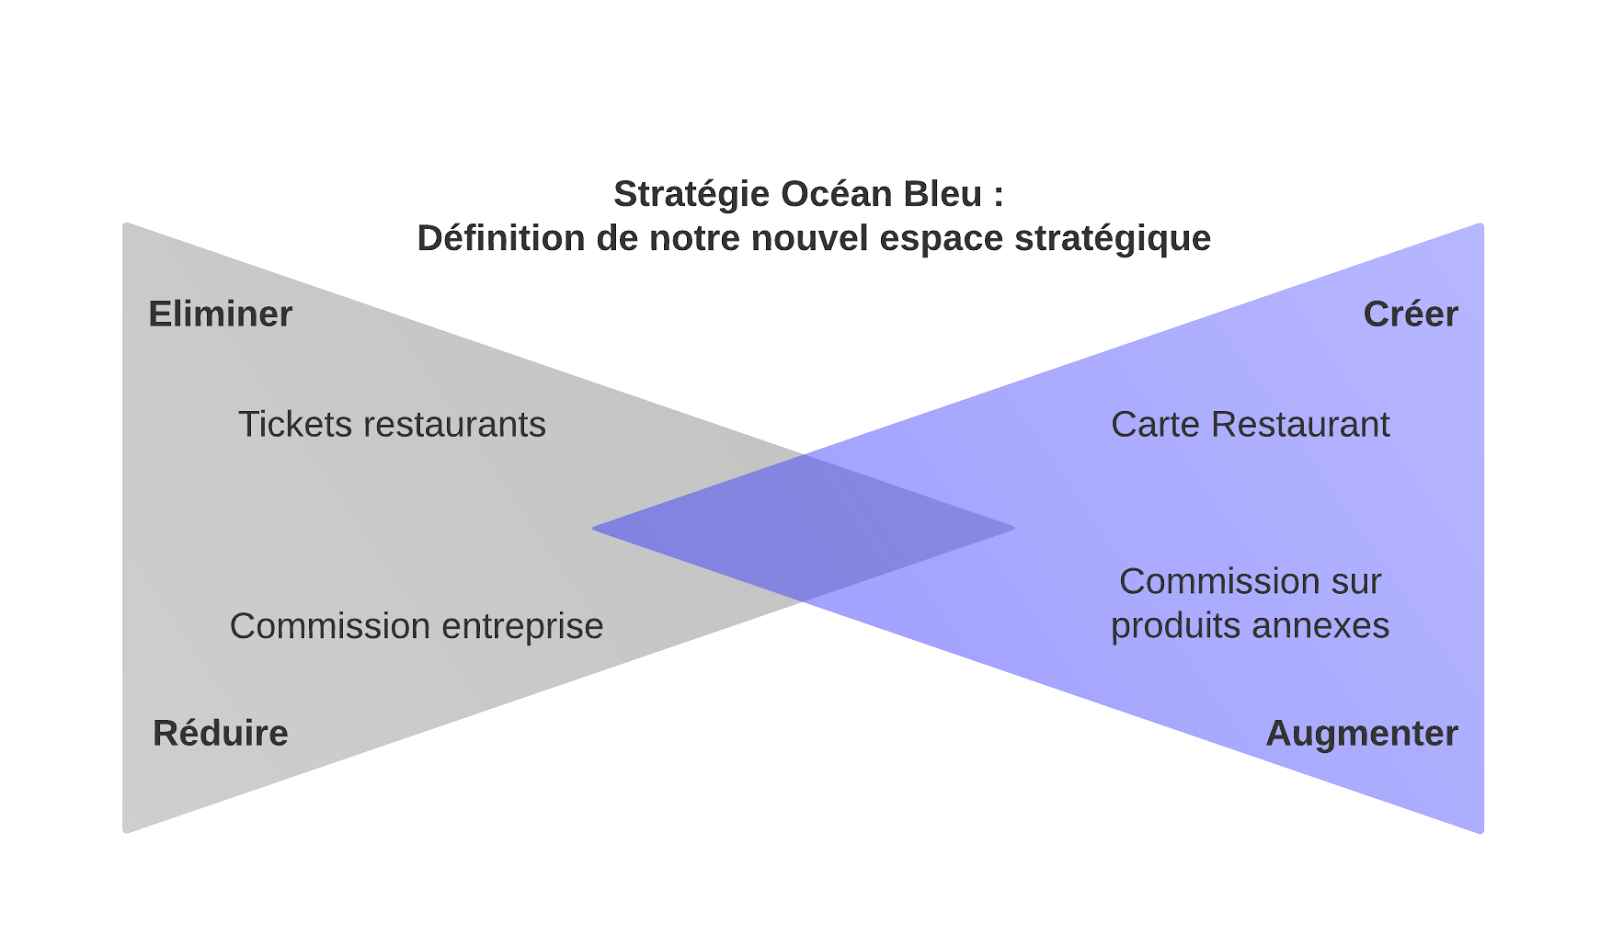
\includegraphics[width=0.8\textwidth]{image05}
    \caption{Stratégie Océan Bleu}
    \label{fig:image05}
\end{figure}

Ce schéma résume notre \textbf{différence avec les A-Players} du marché : notre
proposition 100\% dématérialisée (pure-player). \\

Il montre également la différence fondamentale que nous proposons \textbf{par
rapport aux pure-players} déjà sur le marché en France : notre offre radicale
“0 commission”, pour prendre des parts de marché suffisamment rapidement (cf.
suite). \\

\subsubsection{Canvas}

% \begin{landscape}
  \begin{figure}[htpb]
      \centering
      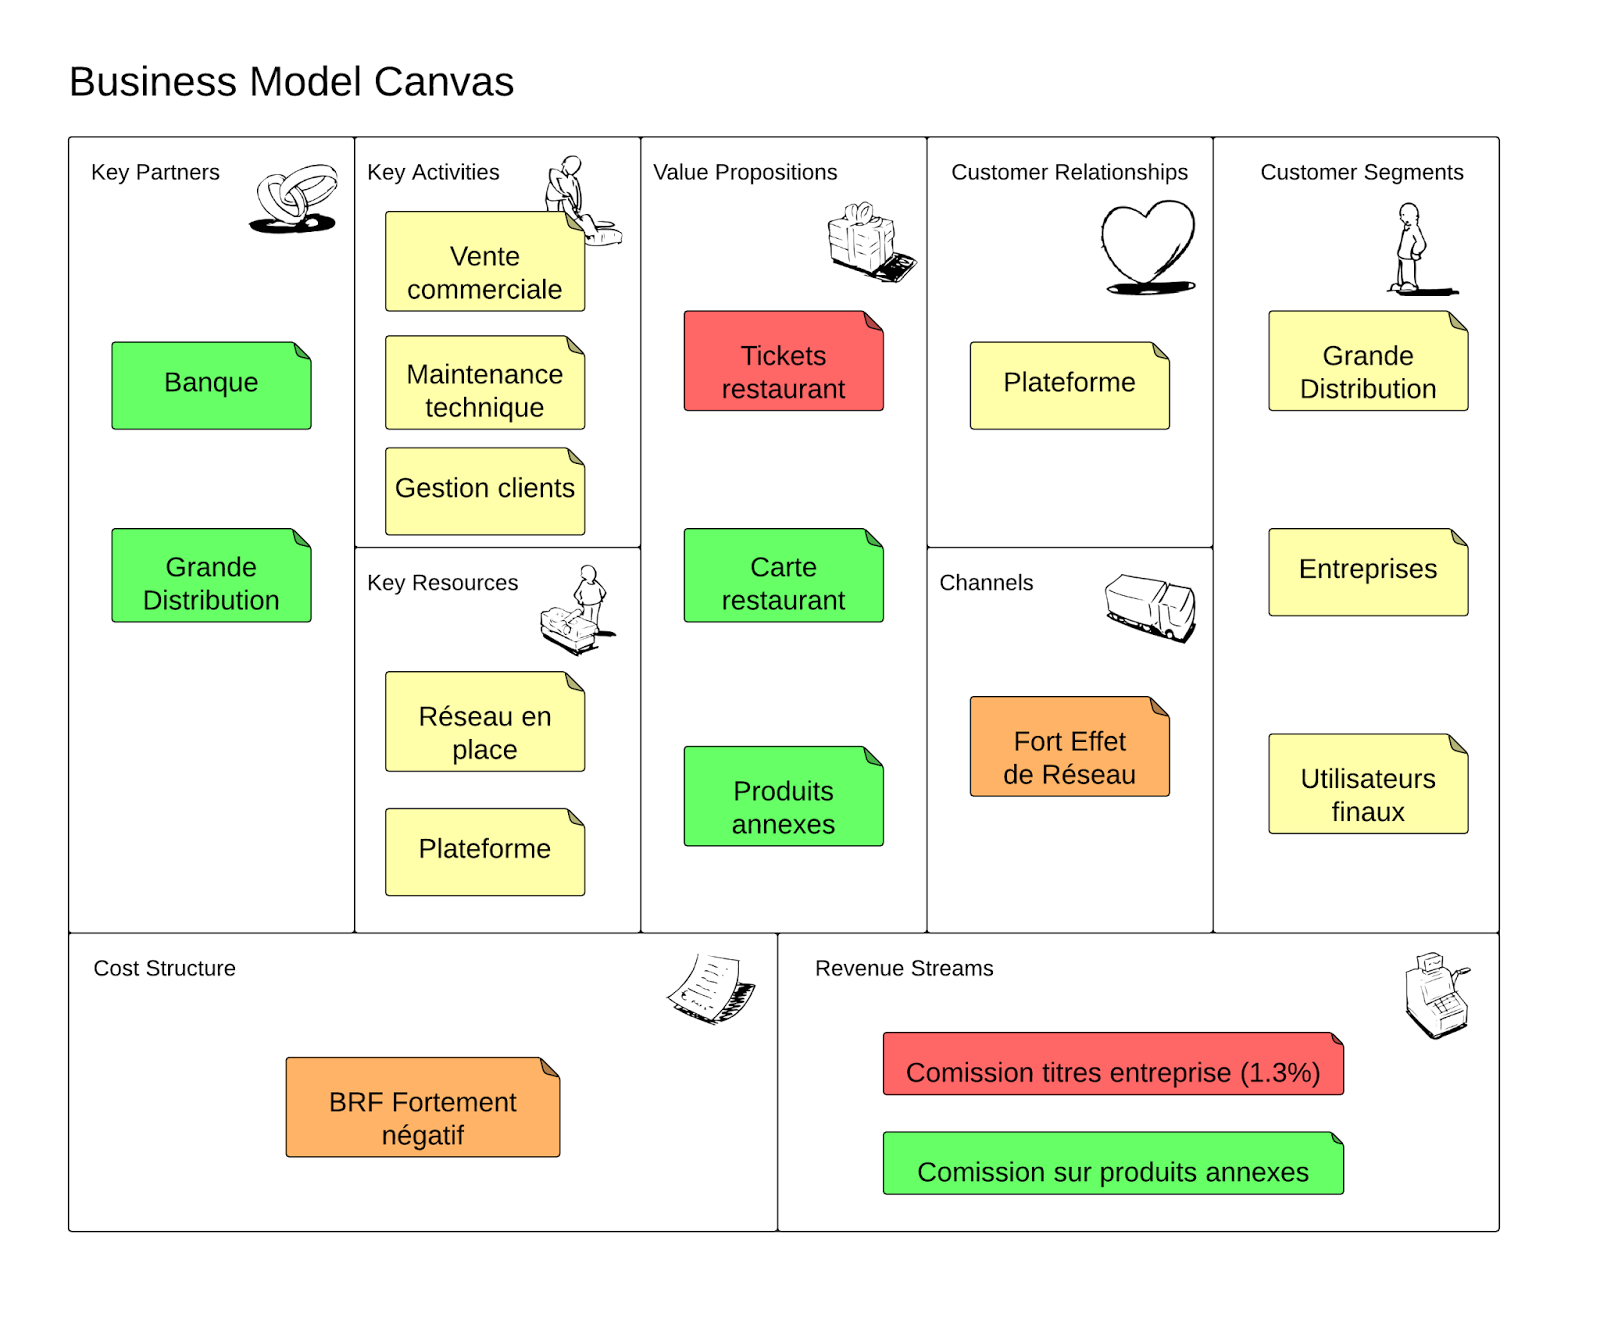
\includegraphics[width=\textwidth]{image00}
      \caption{Détail du business model que nous proposons.
        En vert : les ajouts par rapports au BM classique du milieu.
        En rouge : les retraits que nous effectuons.
        En orange : les barrières à l'entrée principale.
      }
      \label{fig:image00}
  \end{figure}
% \end{landscape}

\subsubsection{Carte restaurant}
Le service que nous proposons est basé sur une carte restaurant, utilisable sur
des terminaux bancaires classiques. La solution n’est pas fondamentalement
différente de celles proposée par Monéo-Resto. Les détails de notre solutions
peuvent être retrouvés dans les autres documents. \\

La \textbf{valeur apportée} par la solution solution dématérialisée
\textbf{n’est plus à prouver}. Son succès unanime dans les pays étrangers en
étant la meilleure preuve. Voici un sondage réalisé sur la l’acceptation des
versions dématérialisées dans les pays qui l’utilisent. L’ensemble des parties
prenantes (entreprises, commerces, salariés) placent tous la variante
dématérialisée loin devant. \\

\begin{figure}[htpb]
    \centering
    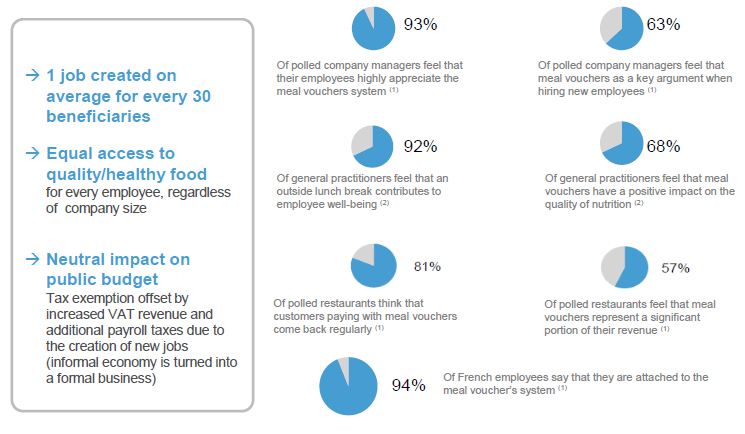
\includegraphics[width=\textwidth]{image03}
    % \caption{}
    % \label{fig:image03}
\end{figure}

\subsubsection{Tickets restaurant}

Nous nous séparons complètement de la solution de paiement par ticket, faisant
de nous un \textbf{“pure-player”}, jouant 100\% sur le dématérialisé. Cela nous
permet de réaliser des \textbf{économies d’échelles} non-négligeables,
fondamentales pour absorber la suppression des commission sur les titres
vendus. \\

\subsubsection{Commission titres entreprise}

Notre approche vis-à-vis des entreprises est radicale : nous prenons \textbf{0
marge} sur la vente des tickets que nous réalisons. \\

Cela représente une économie intéressante pour les entreprises, en particulier
les grandes entreprises, qui pourront réaliser une coupe sur leurs charges (cf.
Projections). \\

Cet \textbf{ajout à notre proposition de valeur} (domination par les coûts)
nous permettra d’acquérir des parts de marchés de manière beaucoup plus rapide,
ce qui est indispensable pour la réussite de l’opération. Cela sous-entend une
force de vente conséquente (cf. Partenariats). \\

\subsubsection{Produits annexes}

La bataille sur les parts de marché long-terme réside donc, en plus de la
stratégie de déploiement que nous allons adopter dans les services que nous
allons créer autour de la carte. \\

Voici la liste de produits annexes que nous envisageons : \\
\begin{itemize}
  \item promotions géolocalisées
  \item e-shopping en partenariat avec des grandes marques
  \item vente des données de consommations collectées (dans le cadre de
    partenariats)
\end{itemize}

\section{Vente \& Marketing}

\begin{figure}[htpb]
    \centering
    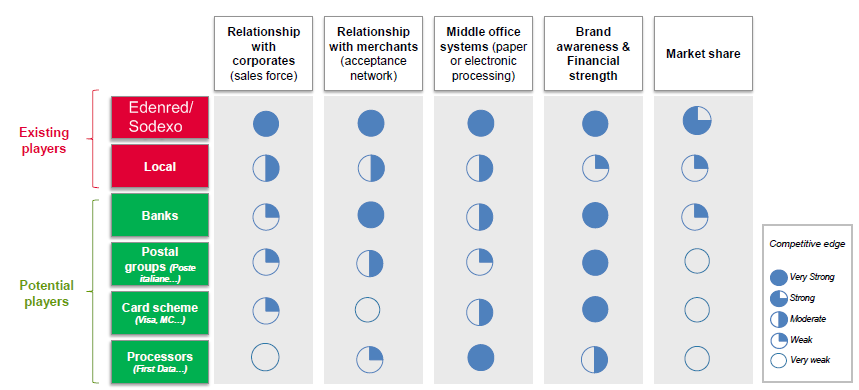
\includegraphics[width=\textwidth]{image04}
    % \caption{}
    % \label{fig:image04}
\end{figure}

% http://investorsanthology.blogspot.fr/2010_06_01_archive.html

\subsection{Partenaires Clés}

\subsubsection{Commerces}

Grandes surfaces de proximité, type “Carrefour City”. \\
Supermarchés périurbains implantés en zone d’activité. \\

Si l’on parvient à nouer un partenariat prospectif avec deux groupes leaders
(par exemple les groupes Carrefour et les Mousquetaires), on peut espérer
s’implanter dans 4-5 000 enseignes la première année, avec 3 ou 4 bornes par
magasin en moyenne. \\

Les restaurateurs (203.000 en France ). Si on se restreint aux enseignes
faciles à démarcher pour la première année (chaînes, gros hubs), on peut tabler
sur 50 000 terminaux de paiement dans autant d’enseignes. \\

\subsection{Caneaux de distribution}

\subsubsection{Client Final}

\subsubsection{Entreprises}

\subsubsection{Commerces}
A chaque fois que l’on signe un nouveau client, on prospecte auprès des
restaurateurs présents aux alentours pour leur proposer de s’affilier. Avant la
mise en place du système, les salariés de l’entreprise sont sondés sur les
endroits où ils utilisent leurs titres-restaurant. Ensuite, on propose à ces
adresses de nous rejoindre \\

\subsection{Activités Clés}
\subsubsection{Technique}

\subsubsection{Commerciale}

\subsection{Ressources Clés}

\subsection{Coûts}
\subsubsection{Investissement}

\subsubsection{Fonctionnement}

\section{Projections}

phase pilote \\

phase de commercialisation \\

Les restaurateurs (203.000 en France ). Si on se restreint aux enseignes
faciles à démarcher pour la première année (chaînes, gros hubs), on peut tabler
sur 50 000 terminaux de paiement dans autant d’enseignes. \\

Pour autant, nous savons déjà que la courbe des commandes ne sera pas linéaire,
car c'est ce qui s'est produit dans tous les autres pays où nous sommes
implantés. Une première vague de clients se montreront intéressés, puis nous
stagnerons à un palier avant que cela ne reparte de façon plus régulière. \\

\begin{figure}[htpb]
    \centering
    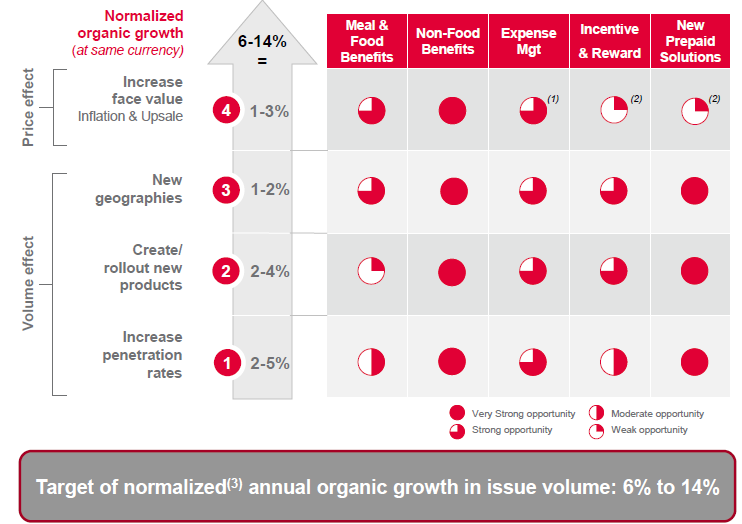
\includegraphics[width=\textwidth]{image01}
    % \caption{}
    % \label{fig:image01}
\end{figure}

\end{document}
